\documentclass[UTF8]{ctexart}
\usepackage{graphicx}                                       % 绘图宏包 for \includegrahpics 命令
\usepackage{xcolor}                                         % 颜色宏包 for 颜色
\usepackage{fancyvrb}                                       % 抄录宏包 for Verbatim 环境
% +++++ 设置页眉页脚 +++++
\usepackage{fancyhdr}
\pagestyle{fancy}
\fancyhf{}
\fancyhead[L]{\fangsong \leftmark}
\fancyhead[R]{\fangsong Tche~L.}
\fancyfoot[C]{\thepage{}}
% -----------------------------------
\usepackage[text={148mm,220mm},centering,includehead,vmarginratio=1:1]{geometry}                    % 设置版面
\setlength{\headwidth}{\textwidth}                          % 设置页眉宽度
\setlength{\headheight}{14pt}                               % 设置页眉高度
% +++++ 设置标题信息 +++++
\title{\vspace{10mm}\heiti\huge 交错网格与完全匹配层\vspace{30mm}}
\author{\LARGE\textsc{Tche~L.}\thanks{~USTC~在读博士,tcheliu@mail.ustc.edu.cn}\vspace{10mm}}
\date{2018年3月1日}
% -----------------------------------
\renewcommand{\thesection}{\chinese{section}、\kern -1em}                                            % 重设节标题
% ++++ 修改节标题格式 ++++
\usepackage{titlesec}
%\titleformat*{\section}{\Large\bf\flushleft}
\titleformat{\section}{\Large\bf\flushleft}{\thesection}{1em}{}%[\vspace{2pt}{\titlerule*[3pt]{\textperiodcentered}}]
%\titleformat{\section}{\titlerule[1pt]\vspace{1pt}\titlerule\vspace{9pt}\bf}{\thesection}{1em}{}[\vspace{6pt}{\titlerule*[3pt]{\textperiodcentered}}]
% -----------------------------------
\usepackage{cite}                                           % 参考文献宏包 for 上标引用
\usepackage{enumerate}                                      % 排序列表宏包 for enumerate 环境
\usepackage{subfig}                                         % 子图宏包 for \subfloat 子图命令
\usepackage{amsmath}										% 公式宏包 for gather 环境
\usepackage{nicefrac}										% 斜分数宏包 for \nicefrac 斜分数命令
\usepackage{amssymb}										% 数学字符宏包 for 黑色方块和三角
\usepackage{listings}
\definecolor{mygrn}{rgb}{0,0.6,0}
\definecolor{mygry}{rgb}{0.5,0.5,0.5}
\definecolor{mymau}{rgb}{0.58,0,0.82}
\usepackage{fontspec}
\lstdefinestyle{Ftsty}{ %
  backgroundcolor=\color{white},
  basicstyle=\scriptsize,
  breakatwhitespace=false,
  breaklines=true,
  captionpos=b,
  commentstyle=\color{mygrn},
  deletekeywords={},
  escapeinside={\%*}{*)},
  extendedchars=true,
  firstnumber=1,
  frame=single,
  keepspaces=true,
  keywordstyle=[1]\color{blue},
  keywordstyle=[2]\color{red},
  language=Fortran,
  morekeywords=[1]{...},
  morekeywords=[2]{InputPara,WaveExtrp,TDFDAWFS2DSG,TDFDEWFS2DSG},
  otherkeywords={NEWUNIT},
  numbers=left,
  numbersep=5pt,
  numberstyle=\tiny\color{mygry},
  rulecolor=\color{black},
  showspaces=false,
  showstringspaces=false,
  showtabs=false,
  stepnumber=5,
  stringstyle=\color{mymau},
  tabsize=2
}
\lstdefinestyle{Mtsty}{ %
  backgroundcolor=\color{white},
  basicstyle=\scriptsize,
  breakatwhitespace=false,
  breaklines=true,
  captionpos=b,
  commentstyle=\color{mygrn},
  deletekeywords={},
  escapeinside={\%*}{*)},
  extendedchars=true,
  firstnumber=1,
  frame=single,
  keepspaces=true,
  keywordstyle=[1]\color{blue},
  keywordstyle=[2]\color{red},
  language=Matlab,
  morekeywords=[1]{...},
  morekeywords=[2]{TDFDAWFS2DSG,TDFDEWFS2DSG},
  otherkeywords={ones},
  numbers=left,
  numbersep=5pt,
  numberstyle=\tiny\color{mygry},
  rulecolor=\color{black},
  showspaces=false,
  showstringspaces=false,
  showtabs=false,
  stepnumber=5,
  stringstyle=\color{mymau},
  tabsize=2
}
\lstdefinestyle{Cpsty}{
  backgroundcolor=\color{white},
  basicstyle=\scriptsize,
  breakatwhitespace=false,
  breaklines=true,
  captionpos=b,
  commentstyle=\color{mygrn},
  deletekeywords={},
  escapeinside={\%*}{*)},
  extendedchars=true,
  firstnumber=1,
  frame=single,
  keepspaces=true,
  keywordstyle=[1]\color{blue},
  keywordstyle=[2]\color{red},
  language=C++,
  morekeywords=[1]{...},
  morekeywords=[2]{TDFDEWFS2DSG},
  otherkeywords={size_t,dim3,ceil,malloc,free,fwrite,__global__,cudaMalloc,cudaMemcpy,cudaFree},
  numbers=left,
  numbersep=5pt,
  numberstyle=\tiny\color{mygry},
  rulecolor=\color{black},
  showspaces=false,
  showstringspaces=false,
  showtabs=false,
  stepnumber=5,
  stringstyle=\color{mymau},
  tabsize=2
}
\renewcommand{\cite}[1]{\textsuperscript{\textsuperscript{\citeleft\citen{#1}\citeright}}}          % 重设参考文献引用格式为上标 [1] 引用
\newcommand{\insertFcode}[2]{\begin{itemize}\item[]\lstinputlisting[caption=#2,label=#1,style=Ftsty]{#1}\end{itemize}}
\newcommand{\insertMcode}[2]{\begin{itemize}\item[]\lstinputlisting[caption=#2,label=#1,style=Mtsty]{#1}\end{itemize}}
\newcommand{\insertCcode}[2]{\begin{itemize}\item[]\lstinputlisting[caption=#2,label=#1,style=Cpsty]{#1}\end{itemize}}
\begin{document}

\maketitle
\centerline{Version: 2.2}
\vspace{50mm}

有限差分法是对介质模型,也就是对计算区域先进行离散网格化,将描述介质中传播的波动微分方程,利用微商和差商的近似关系,直接化为有限差分方程来求解,模拟波的传播。\par
地震勘探中的有限差分根据域的不同可分为时域有限差分和频域有限差分。根据网格不同可分为同位网格\cite{Alterman_1968}、交错网格\cite{Virieux_1984}\cite{Virieux_1986}、旋转网格\cite{Saenger_2000}\cite{Saenger_2004}等。对于边界反射波的处理,有早期的旁轴近似吸收边界条件\cite{Clayton_1977}、指数型吸收边界条件\cite{Cerjan_1985}和现在比较流行的完全匹配层吸收边界\cite{Collino_2001}。
本文主要介绍了时域交错网格有限差分方法与完全匹配层吸收边界条件,并对简单的二维声波方程和弹性波方程给出了差分格式。\par

\newpage

\section{什么是交错网格}
交错网格是将不同的地震波场分量定义在整网格点和半网格点上,合理地安排地震波场分量在网格上的相对位置,可以方便地求取所需分量的差分。同时,它将波场分裂为~$x$~和~$z$~方向上的两个分量,将二阶位移微分方程分裂为若干个一阶速度—应力方程对波场进行求解。在交错网格中,假设~$u^x$~和~$u^z$~分别定义在~$x$~和~$z$~方向的半网格点上,则它们对~$x$~和~$z$~方向的中心差分格式为\cite{sun_2013}
\begin{equation}
\left\{ \begin{aligned}
& L_x(u^x_{i,j})=\frac{1}{\Delta x}\sum_{n=1}^{N}C_n^{(N)}(u^x_{i+\frac{2n-1}{2},j}-u^x_{i-\frac{2n-1}{2},j}) \\
& L_z(u^z_{i,j})=\frac{1}{\Delta z}\sum_{n=1}^{N}C_n^{(N)}(u^z_{i,j+\frac{2n-1}{2}}-u^z_{i,j-\frac{2n-1}{2}})
\end{aligned} \right.
\end{equation}
其中,$u$~为地震波场值,$u^x$~和~$u^z$~为它的两个方向分量,$\Delta x$~和~$\Delta z$~为~$x$~和~$z$~方向的空间间隔,$C_n^{(N)}$~为差分系数,$2N$~为差分的空间阶数。\par

\section{什么是完全匹配层}
吸收边界条件的思想就是在需要计算场值的区域之外加上一定厚度的吸收边界层,当波运行到计算边界时候,不会发生反射,而是直接穿透边界进入所加的吸收边界层,对吸收边界层设置一定的参数,从而起到吸收超出边界的波的作用。\par
\begin{figure}[h]
  \centering
  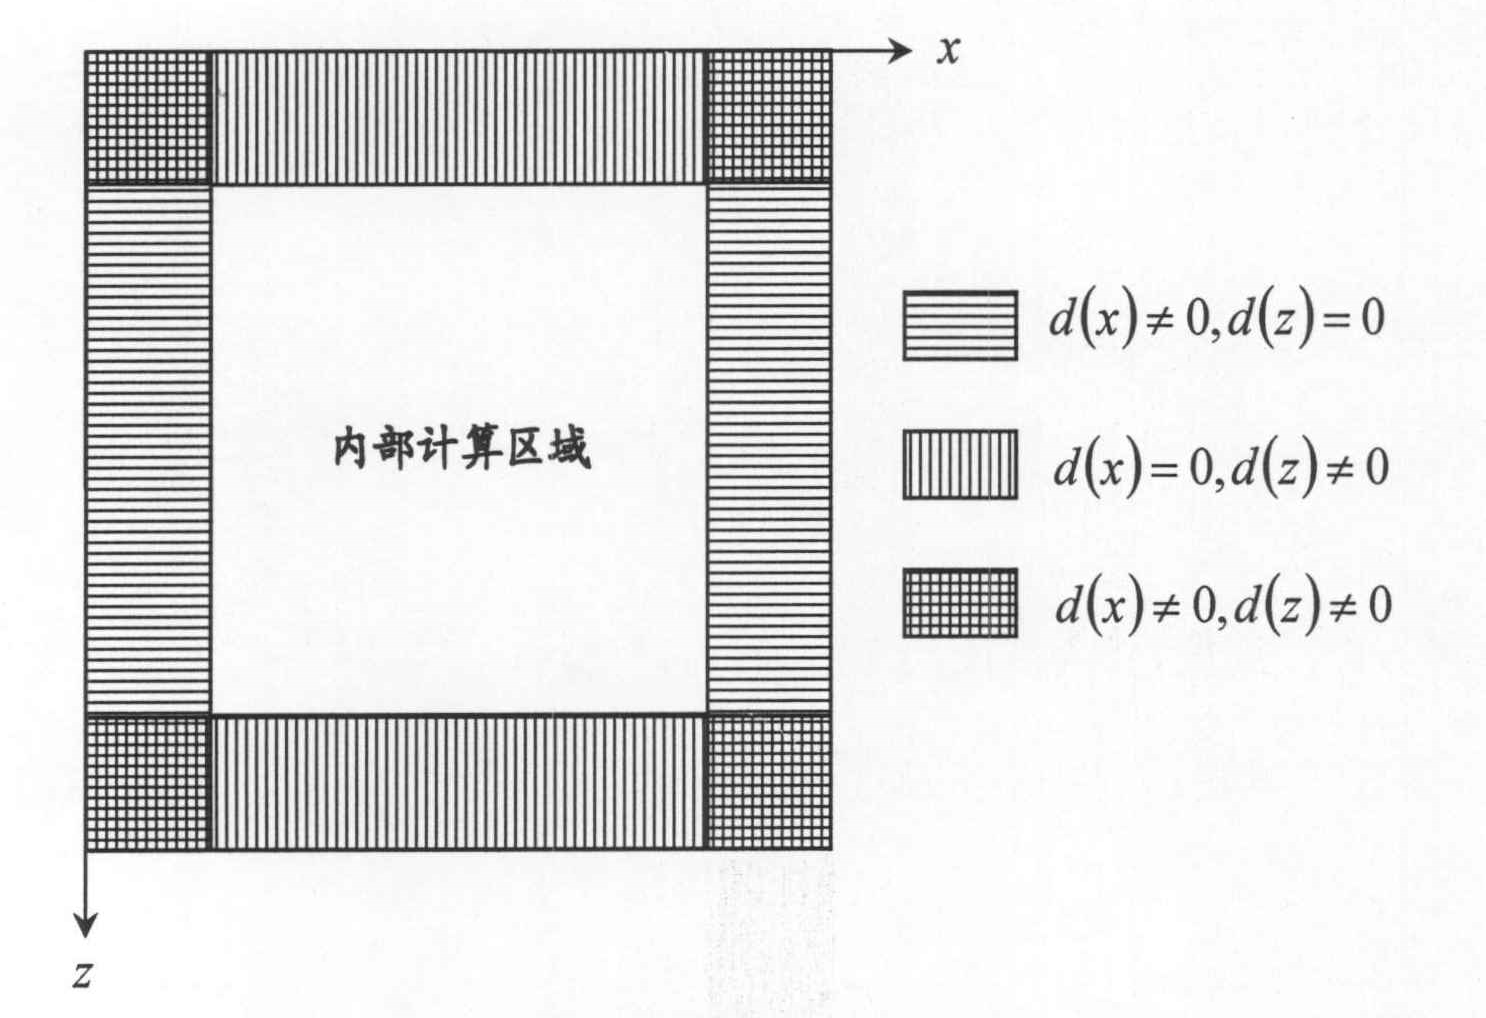
\includegraphics[width=90mm]{./Figure/pml.png}
  \caption{完全匹配层吸收边示意图(图中:$d(x)=d_x,~d(z)=d_z$)}\label{fig:pml}
\end{figure}
在时域有限差分方法波场模拟中,完全匹配层(PML)吸收边界条件将波场分量在吸收边界区域分裂,分别对各个分裂的波场分量赋以不同的耗损。在计算区域截断边界外,PML~层是一种非物理的特殊吸收介质,该层的波阻抗与相邻介质的波阻抗完全匹配,因而入射波将无反射地穿过界面进行~PML~层,同时,由于~PML~层为有耗介质,进入~PML~层的入射波将迅速衰减,最终实现消弱边界反射的效果。\par
PML~吸收边界具体做法如图~\ref{fig:pml}~所示,在内部计算区域,采用一般的速度—应力方程,而在~PML~层区域内,在频率空间域对方程中的~$x$~和~$z$~方向偏导分别作如下替换:
\[ \frac{\partial}{\partial x}\longrightarrow\frac{i\omega}{i\omega+d_x}\frac{\partial}{\partial x},\hspace{20mm} \frac{\partial}{\partial z}\longrightarrow\frac{i\omega}{i\omega+d_z}\frac{\partial}{\partial z} \]
其中,$\omega$~为角频率,$d_x$~和~$d_z$~分别为~$x$~和~$z$~方向的阻尼因子。\par
例如,对于如下方程:
\[ \frac{\partial u}{\partial t}=A\frac{\partial v}{\partial x} \]
在内部计算区域,我们采用上式求解即可。而在~PML~层内,我们应对方程作一些调整。上式对应的频率空间域方程为:
\[ i\omega u=A\frac{\partial v}{\partial x} \]
在~PML~层内,对~$x$~方向偏导进行替换,得到如下方程:
\[ i\omega u=A\frac{i\omega}{i\omega+d_x}\frac{\partial v}{\partial x} \text{,也即~} (i\omega+d_x)u=A\frac{\partial v}{\partial x} \]
其在时间空间域的表达形式为:
\begin{equation}\label{eq:dpml}
\Big(\frac{\partial}{\partial t}+d_x\Big)u=A\frac{\partial v}{\partial x}
\end{equation}
因此,我们在~PML~层内可采用上式求解,即可实现~PML~吸收边界层内衰减。\par
在对上式左侧采用差分近似的实际过程中,我们有两种近似方案。先假设上式右侧经空间差分近似后的结果为
\[ A\dfrac{\partial v_k}{\partial x}\approx\spadesuit|_k \]
其中~$\partial v_k$~为~$k\Delta t$~时刻~$v$~的偏导,$\Delta t$~为时间步长。同时假设~$u$~定义在半时间网格点上,则第一种近似方案为:
\[ \Big(\frac{\partial}{\partial t}+d_x\Big)u_k=\frac{\partial u_k}{\partial t}+d_x\cdot u_k=\frac{u_{k+\nicefrac{1}{2}}-u_{k-\nicefrac{1}{2}}}{\Delta t}+d_x\cdot\frac{u_{k+\nicefrac{1}{2}}+u_{k-\nicefrac{1}{2}}}{2} \]
将上式代入式~\eqref{eq:dpml},最终,我们得到第一种近似下的时间递推关系式为:
\begin{equation}\label{eq:pml1}
u_{k+\nicefrac{1}{2}}=\frac{2-\Delta t\cdot d_x}{2+\Delta t\cdot d_x}\cdot u_{k-\nicefrac{1}{2}}+\frac{2\Delta t}{2+\Delta t\cdot d_x}\cdot\spadesuit|_k
\end{equation}
第二种近似方案为:
\[ \Big(\frac{\partial}{\partial t}+d_x\Big)u_k=\frac{\partial u_k}{\partial t}+d_x\cdot u_k=\frac{u_{k+\nicefrac{1}{2}}-u_{k-\nicefrac{1}{2}}}{\Delta t}+d_x\cdot u_{k-\nicefrac{1}{2}} \]
将其代入式~\eqref{eq:dpml},最终,我们得到第二种近似下的时间递推关系式为:
\begin{equation}\label{eq:pml2}
u_{k+\nicefrac{1}{2}}=\big(1-\Delta t\cdot d_x\big)u_{k-\nicefrac{1}{2}}+\Delta t\cdot\spadesuit|_k
\end{equation}\par
其实,我们可以将内部计算区域和~PML~层区域的方程统一起来,当~$d_x=d_z=0$~时~PML~层区域的方程转化为内部计算区域的方程,编程时我们可以考虑统一采用~PML~层区域的方程形式求解,只需特别地在内部计算区域令~$d_x=d_z=0$~即可。\par
那么,衰减因子~$d_x$~和~$d_z$~如何给定?对于上边界或左边界,文献\cite{Marcinkovich_2003}给出了形如下式的衰减因子:
\[ d_*(i)=d_{0*}\Big(\frac{i}{n_{pml*}}\Big)^p \]
其中,$*$~表示~$x$~或~$z$,$i$~为从内部有效计算区域边界起算的~PML~层数,$n_{pml*}$~为在~$*$~方向上所加载的单边~PML~层网格点数,典型地~$p$~的取值范围为~$1\sim4$。另外,
\[ d_{0*}=\log\Big(\frac{1}{R}\Big)\frac{\tau V_s}{n_{pml*}\Delta *} \]
或
\[ d_{0*}=\frac{\tau V_s}{\Delta *}\big(c_1+c_2 n_{pml*}+c_3 n_{pml*}^2\big) \]
其中,$R$~为理论反射系数;$\tau$~为微调参数,取值范围为~$3\sim4$;$V_s$~为横波波速;$\Delta *$~为在~$*$~方向上的网格间距;$c_i$~为多项式系数。对于~$R$~或~$c_i$~的取值如下:
\[ \left\{ \begin{aligned}
& R=0.01,   & \hspace{5mm} & \text{当}~n_{pml*}=5 \\
& R=0.001,  & \hspace{5mm} & \text{当}~n_{pml*}=10 \\
& R=0.0001, & \hspace{5mm} & \text{当}~n_{pml*}=20
\end{aligned} \right.
\hspace{10mm}\text{或}\hspace{10mm}
\left\{ \begin{aligned}
& c_1=\frac{8}{15} \\
& c_2=\frac{-3}{100} \\
& c_3=\frac{1}{1500}
\end{aligned} \right. \]\par

\section{空间上任意偶数阶差分近似}
在交错网格方法中,波场分量的导数是在相应的分量网格节点之间的半程上计算的。因此,我们可以用下式计算方程中的一阶空间导数:
\begin{equation}\label{eq:dudx}
\frac{\partial u}{\partial x}=\frac{1}{\Delta x}\sum_{n=1}^N\Big\{C_n^{(N)}\big[u\big(x+\frac{2n-1}{2}\Delta x\big)-u\big(x-\frac{2n-1}{2}\Delta x\big)\big]\Big\}+O\big(\Delta x^{2N}\big)
\end{equation}
上式中待定系数~$C_n^{(N)}$~的准确求取是确保一阶空间导数的~$2N$~阶差分精度的关键。将~$u\big(x+\frac{2n-1}{2}\Delta x\big)$~和~$u\big(x-\frac{2n-1}{x}\Delta x\big)$~在~$x$~处~Taylor~展开后可以发现,通过求解下列方程组即可确定待定系数~$C_n^{(N)}$:
\[ \left[ \begin{array}{c@{}c@{}c@{}c@{}c}
1^1      & 3^1      & 5^1      & \cdots & (2N-1)^1      \\
1^3      & 3^3      & 5^3      & \cdots & (2N-1)^3      \\
1^5      & 3^5      & 5^5      & \cdots & (2N-1)^5      \\
\vdots   & \vdots   & \vdots   & \ddots & \vdots        \\
1^{2N-1} & 3^{2N-1} & 5^{2N-1} & \cdots & (2N-1)^{2N-1}
\end{array}\right]
\left[\begin{array}{c}
C_1^{(N)} \\
C_2^{(N)} \\
C_3^{(N)} \\
\vdots    \\
C_N^{(N)} \\
\end{array}\right]=
\left[\begin{array}{c}
1      \\
0      \\
0      \\
\vdots \\
0      \\
\end{array} \right] \]
其解为:
\begin{equation}
C_m^{(N)}=\frac{(-1)^{m+1}\prod\limits_{i=1,i\neq m}^N(2i-1)^2}{(2m-1)\prod\limits_{i=1,i\neq m}^N\big|(2m-1)^2-(2i-1)^2\big|}
\end{equation}\par

\section{交错网格中的声波方程}
如我们所常见的,在各向同性介质中,二维声波波动方程可表示为:
\begin{equation}\label{eq:awave}
\frac{\partial^2 P}{\partial t^2}=v_P^2\Big(\frac{\partial^2 P}{\partial x^2}+\frac{\partial^2 P}{\partial z^2}\Big)
\end{equation}
其中,$P$~为压力波场或位移波场,$v_P$~为介质声波波速。\par
在交错网格中,我们将不同的波场分量定义在不同的网格点上,这就需要我们采用多波场分量的方程来进行波场模拟。在各向同性介质中,二维声波一阶速度—应力方程可表示为:
\begin{equation}\label{eq:awuv}
\left\{ \begin{aligned}
& \frac{\partial P}{\partial t}=-\rho v_P^2 \big(\frac{\partial v_x}{\partial x}+\frac{\partial v_z}{\partial z} \big) \\
& \frac{\partial v_x}{\partial t}=-\frac{1}{\rho} \frac{\partial P}{\partial x} \\
& \frac{\partial v_z}{\partial t}=-\frac{1}{\rho} \frac{\partial P}{\partial z}
\end{aligned} \right.
\end{equation}
其中,$v_x$~和~$v_z$~分别为在~$x$~和~$z$~方向的质点运动速度波场分量,$\rho$~为介质密度。\par
在方程~\eqref{eq:awuv}~中的第一个等式两边同时对~$t$~求偏导,交换等式右侧对时间求导和对空间求导的先后顺序,再结合方程~\eqref{eq:awuv}~中的后两个等式,即可得到如式~\eqref{eq:awave}~所示的波动方程。\par
在~PML~吸收边界中,我们在~$x$~和~$z$~方向上采取不同的阻尼衰减因子,由于方程~\eqref{eq:awuv}~中的第一个等式同时包含了对~$x$~和~$z$~方向的偏导,因此,还需要对该式作进一步拆分:
\begin{equation}\label{eq:Pxz}
\left\{ \begin{aligned}
& P=P_x+P_z \\
& \frac{\partial P_x}{\partial t}=-\rho v_P^2 \frac{\partial v_x}{\partial x} \\
& \frac{\partial P_z}{\partial t}=-\rho v_P^2 \frac{\partial v_z}{\partial z}
\end{aligned} \right.
\end{equation}
其中,$P_x$~和~$P_z$~分别为应力波场~$P$~在~$x$~和~$z$~方向上的分量。\par
根据式~\eqref{eq:awuv}~和~\eqref{eq:Pxz}~,引入~PML~吸收边界条件,得到:
\begin{equation}
\left\{ \begin{aligned}
& \big(\frac{\partial}{\partial t}+d_x\big)v_x=-\frac{1}{\rho}\frac{\partial P}{\partial x} \\
& \big(\frac{\partial}{\partial t}+d_z\big)v_z=-\frac{1}{\rho}\frac{\partial P}{\partial z} \\
& \big(\frac{\partial}{\partial t}+d_x\big)P_x=-\rho v_P^2\frac{\partial v_x}{\partial x} \\
& \big(\frac{\partial}{\partial t}+d_z\big)P_z=-\rho v_P^2\frac{\partial v_z}{\partial z}
\end{aligned} \right.
\end{equation}\par
\begin{figure}[t]
  \centering
  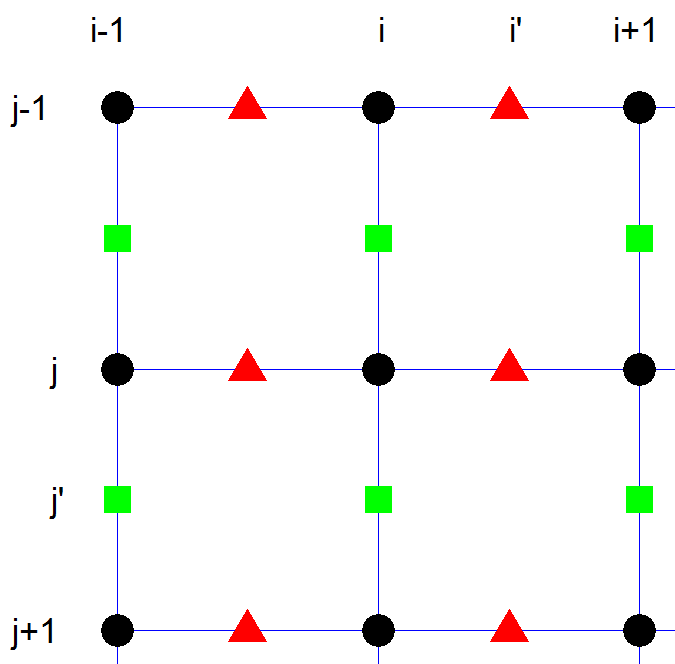
\includegraphics[width=70mm]{./Figure/asg.png}
  \caption{声波交错网格示意图($\bullet$:$P,~\rho v_P^2$;{\color{red}$\blacktriangle$}:$v_x,~\nicefrac{1}{\rho}$;{\color{green}$\blacksquare$}:$v_z,~\nicefrac{1}{\rho}$)}\label{fig:asg}
\end{figure}
按照如图~\ref{fig:asg}~所示波场分量和参数排布方式,我们在时间上采用如式~\eqref{eq:pml2}~所示的递推格式,在空间上采用如式~\eqref{eq:dudx}~所示的任意偶数阶差分近似,可以得到在~PML~层内采用第二种近似下的时间二阶差分精度、空间~$2N$~阶差分精度的交错网格有限差分声波方程时间递推格式如下:
\begin{equation}
\left\{ \begin{aligned}
& v_x\big|_{i+\nicefrac{1}{2},j}^k=\big(1-\Delta t\cdot d_x\big) v_x\big|_{i+\nicefrac{1}{2},j}^{k-1}-\frac{\Delta t}{\rho\Delta x}\sum\limits_{n=1}^N\Big\{C_n^{(N)}\big[P\big|_{i+\nicefrac{1}{2}+\nicefrac{(2n-1)}{2},j}^{k-\nicefrac{1}{2}}-P\big|_{i+\nicefrac{1}{2}-\nicefrac{(2n-1)}{2},j}^{k-\nicefrac{1}{2}}\big]\Big\} \\
& v_z\big|_{i,j+\nicefrac{1}{2}}^k=\big(1-\Delta t\cdot d_z\big) v_z\big|_{i,j+\nicefrac{1}{2}}^{k-1}-\frac{\Delta t}{\rho\Delta z}\sum\limits_{n=1}^N\Big\{C_n^{(N)}\big[P\big|_{i,j+\nicefrac{1}{2}+\nicefrac{(2n-1)}{2}}^{k-\nicefrac{1}{2}}-P\big|_{i,j+\nicefrac{1}{2}-\nicefrac{(2n-1)}{2}}^{k-\nicefrac{1}{2}}\big]\Big\} \\
& P_x\big|_{i,j}^{k+\nicefrac{1}{2}}=\big(1-\Delta t\cdot d_x\big) P_x\big|_{i,j}^{k-\nicefrac{1}{2}}-\frac{\rho v_P^2\Delta t}{\Delta x}\sum\limits_{n=1}^N\Big\{C_n^{(N)}\big[v_x\big|_{i+\nicefrac{(2n-1)}{2},j}^k-v_x\big|_{i-\nicefrac{(2n-1)}{2},j}^k\big]\Big\} \\
& P_z\big|_{i,j}^{k+\nicefrac{1}{2}}=\big(1-\Delta t\cdot d_z\big) P_z\big|_{i,j}^{k-\nicefrac{1}{2}}-\frac{\rho v_P^2\Delta t}{\Delta z}\sum\limits_{n=1}^N\Big\{C_n^{(N)}\big[v_z\big|_{i,j+\nicefrac{(2n-1)}{2}}^k-v_z\big|_{i,j-\nicefrac{(2n-1)}{2}}^k\big]\Big\}
\end{aligned} \right.
\end{equation}
其中,$P=P_x+P_z$,$v_x\big|_{i+\nicefrac{1}{2},j}^k$~为空间网格点~$\big((i+\nicefrac{1}{2})\Delta x,j\Delta z\big)$~处在~$k\Delta t$~时刻~$v_x$~的值,$\Delta x$~和~$\Delta z$~分别为~$x$~和~$z$~方向上空间差分步长。\par

\section{交错网格中的弹性波方程}
对于弹性波方程,如我们所常见的,在各向同性介质中,二维波动方程可表示为:
\begin{equation}\label{eq:ewave}
\left\{ \begin{aligned}
& \rho \frac{\partial^2 u_x}{\partial t^2}=\frac{\partial}{\partial x}\big[\lambda\big(\frac{\partial u_x}{\partial x}+\frac{\partial u_z}{\partial z}\big)+2\mu\frac{\partial u_x}{\partial x}\big]+\frac{\partial}{\partial z}\big[\mu\big(\frac{\partial u_z}{\partial x}+\frac{\partial u_x}{\partial z}\big)\big] \\
& \rho \frac{\partial^2 u_z}{\partial t^2}=\frac{\partial}{\partial z}\big[\lambda\big(\frac{\partial u_x}{\partial x}+\frac{\partial u_z}{\partial z}\big)+2\mu\frac{\partial u_z}{\partial z}\big]+\frac{\partial}{\partial x}\big[\mu\big(\frac{\partial u_z}{\partial x}+\frac{\partial u_x}{\partial z}\big)\big]
\end{aligned} \right.
\end{equation}
其中,$u_x$~和~$u_z$~分别为~$x$~和~~$z$~方向上的位移,$\rho$~为介质密度,$\lambda=\rho(v_p^2-2v_s^2)$~和~$\mu=\rho v_s^2$~为介质拉梅常数,$v_p$~和~$v_s$~分别为介质的纵波速度和横波速度。\par
另外,我们有弹性动力学方程如下\cite{Virieux_1986}:
\begin{equation}\label{eq:ewut}
\left\{ \begin{aligned}
& \rho \frac{\partial^2 u_x}{\partial t^2}=\frac{\partial \tau_{xx}}{\partial x}+\frac{\partial \tau_{xz}}{\partial z} \\
& \rho \frac{\partial^2 u_z}{\partial t^2}=\frac{\partial \tau_{xz}}{\partial x}+\frac{\partial \tau_{zz}}{\partial z} \\
& \tau_{xx}=(\lambda+2\mu)\frac{\partial u_x}{\partial x}+\lambda\frac{\partial u_z}{\partial z} \\
& \tau_{zz}=(\lambda+2\mu)\frac{\partial u_z}{\partial z}+\lambda\frac{\partial u_x}{\partial x} \\
& \tau_{xz}=\mu\big(\frac{\partial u_x}{\partial z}+\frac{\partial u_z}{\partial x}\big)
\end{aligned} \right.
\end{equation}
其中,$(\tau_{xx},\tau_{zz},\tau_{xz})$~为应力张量。不难发现,我们将方程~\eqref{eq:ewut}~的后三个等式代入前两个等式中,即可得到如式~\eqref{eq:ewave}~所示的波动方程。\par
然而,仅有上式,由于含有对时间的二阶偏导项,我们并不能将~PML~吸收边界条件直接引进来。我们将质点运动速度波场分量~$v_x=\nicefrac{\partial u_x}{\partial t}$~和~$v_z=\nicefrac{\partial u_z}{\partial t}$~引入上式,得到如下二维弹性波一阶速度—应力方程:
\begin{equation}
\left\{ \begin{aligned}
& \frac{\partial v_x}{\partial t}=\frac{1}{\rho}\big(\frac{\partial \tau_{xx}}{\partial x}+\frac{\partial \tau_{xz}}{\partial z}\big) \\
& \frac{\partial v_z}{\partial t}=\frac{1}{\rho}\big(\frac{\partial \tau_{xz}}{\partial x}+\frac{\partial \tau_{zz}}{\partial z}\big) \\
& \frac{\partial \tau_{xx}}{\partial t}=(\lambda+2\mu)\frac{\partial v_x}{\partial x}+\lambda\frac{\partial v_z}{\partial z} \\
& \frac{\partial \tau_{zz}}{\partial t}=(\lambda+2\mu)\frac{\partial v_z}{\partial z}+\lambda\frac{\partial v_x}{\partial x} \\
& \frac{\partial \tau_{xz}}{\partial t}=\mu\big(\frac{\partial v_x}{\partial z}+\frac{\partial v_z}{\partial x} \big)
\end{aligned} \right.
\end{equation}\par
但是,由于上式的每一个等式中都同时含有对~$x$~和~$z$~的偏导,依然不能直接引入~PML~边界条件。接下来,我们需要对上式中的每一个等式作如式~\eqref{eq:Pxz}~所示的拆分,进一步得到:
\begin{equation}
\left\{ \begin{aligned}
& v_x=v_x^x+v_x^z, & \hspace{5mm} & \frac{\partial v_x^x}{\partial t}=\frac{1}{\rho}\frac{\partial \tau_{xx}}{\partial x}, & \hspace{5mm} & \frac{\partial v_x^z}{\partial t}=\frac{1}{\rho}\frac{\partial \tau_{xz}}{\partial z} \\
& v_z=v_z^x+v_z^z, & \hspace{5mm} & \frac{\partial v_z^x}{\partial t}=\frac{1}{\rho}\frac{\partial \tau_{xz}}{\partial x}, & \hspace{5mm} & \frac{\partial v_z^z}{\partial t}=\frac{1}{\rho}\frac{\partial \tau_{zz}}{\partial z} \\
& \tau_{xx}=\tau_{xx}^x+\tau_{xx}^z, & \hspace{5mm} & \frac{\partial \tau_{xx}^x}{\partial t}=(\lambda+2\mu)\frac{\partial v_x}{\partial x}, & \hspace{5mm} & \frac{\partial \tau_{xx}^z}{\partial t}=\lambda\frac{\partial v_z}{\partial z} \\
& \tau_{zz}=\tau_{zz}^x+\tau_{zz}^z, & \hspace{5mm} & \frac{\partial \tau_{zz}^x}{\partial t}=\lambda\frac{\partial v_x}{\partial x}, & \hspace{5mm} & \frac{\partial \tau_{zz}^z}{\partial t}=(\lambda+2\mu)\frac{\partial v_z}{\partial z} \\
& \tau_{xz}=\tau_{xz}^x+\tau_{xz}^z, & \hspace{5mm} & \frac{\partial \tau_{xz}^x}{\partial t}=\mu\frac{\partial v_z}{\partial x}, & \hspace{5mm} & \frac{\partial \tau_{xz}^z}{\partial t}=\mu\frac{\partial v_x}{\partial z}
\end{aligned} \right.
\end{equation}\par
至此,我们可以在上式的时间微分中引入~PML~层吸收边界,得到:
\begin{equation}
\left\{ \begin{aligned}
& \big(\frac{\partial}{\partial t}+d_x\big)v_x^x=\frac{1}{\rho}\frac{\partial \tau_{xx}}{\partial x}, & \hspace{10mm} & \big(\frac{\partial}{\partial t}+d_z\big)v_x^z=\frac{1}{\rho}\frac{\partial \tau_{xz}}{\partial z} \\
& \big(\frac{\partial}{\partial t}+d_x\big)v_z^x=\frac{1}{\rho}\frac{\partial \tau_{xz}}{\partial x}, & \hspace{10mm} & \big(\frac{\partial}{\partial t}+d_z\big)v_z^z=\frac{1}{\rho}\frac{\partial \tau_{zz}}{\partial z} \\
& \big(\frac{\partial}{\partial t}+d_x\big)\tau_{xx}^x=\big(\lambda+2\mu\big)\frac{\partial v_x}{\partial x}, & \hspace{10mm} & \big(\frac{\partial}{\partial t}+d_z\big)\tau_{xx}^z=\lambda\frac{\partial v_z}{\partial z} \\
& \big(\frac{\partial}{\partial t}+d_x\big)\tau_{zz}^x=\lambda\frac{\partial v_x}{\partial x}, & \hspace{10mm} & \big(\frac{\partial}{\partial t}+d_z\big)\tau_{zz}^z=\big(\lambda+2\mu\big)\frac{\partial v_z}{\partial z} \\
& \big(\frac{\partial}{\partial t}+d_x\big)\tau_{xz}^x=\mu\frac{\partial v_z}{\partial x}, & \hspace{10mm} & \big(\frac{\partial}{\partial t}+d_z\big)\tau_{xz}^z=\mu\frac{\partial v_x}{\partial z}
\end{aligned} \right.
\end{equation}
其中,
\begin{equation}\label{eq:vt+}
\left\{ \begin{aligned}
& v_x=v_x^x+v_x^z \\
& v_z=v_z^x+v_z^x \\
& \tau_{xx}=\tau_{xx}^x+\tau_{xx}^z \\
& \tau_{zz}=\tau_{zz}^x+\tau_{zz}^z \\
& \tau_{xz}=\tau_{xz}^x+\tau_{xz}^z
\end{aligned} \right.
\end{equation}\par
\begin{figure}[t]
  \centering
  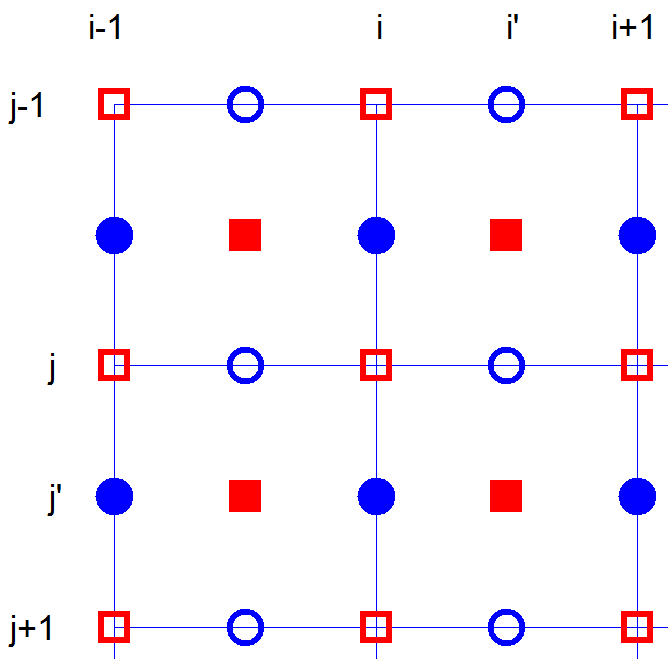
\includegraphics[width=70mm]{./Figure/esg.png}
  \caption{弹性波交错网格示意图({\color{red}$\square$}:$v_x,~\nicefrac{1}{\rho}$;{\color{red}$\blacksquare$}:$v_z,~\nicefrac{1}{\rho}$;{\color{blue}$\circ$}:$\tau_{xx},~\tau_{zz},~(\lambda+2\mu),~\lambda$;{\color{blue}$\bullet$}:$\tau_{xz},~\mu$)}\label{fig:esg}
\end{figure}
按照如图~\ref{fig:esg}~所示波场分量和参数排布方式,我们在时间上采用如式~\eqref{eq:pml2}~所示的递推格式,在空间上采用如式~\eqref{eq:dudx}~所示的任意偶数阶差分近似,可以得到在~PML~层内采用第二种近似下的时间二阶差分精度、空间~$2N$~阶差分精度的交错网格有限差分弹性波方程时间递推格式如下:
\begin{equation}
\left\{ \begin{aligned}
& v_x^x\big|_{i,j}^{k+\nicefrac{1}{2}}=\big(1-\Delta t\cdot d_x\big) v_x^x\big|_{i,j}^{k-\nicefrac{1}{2}}+\frac{\Delta t}{\rho\Delta x}\sum\limits_{n=1}^N\Big\{C_n^{(N)}\big[\tau_{xx}\big|_{i+\nicefrac{(2n-1)}{2},j}^k-\tau_{xx}\big|_{i-\nicefrac{(2n-1)}{2},j}^k\big]\Big\} \\
& v_x^z\big|_{i,j}^{k+\nicefrac{1}{2}}=\big(1-\Delta t\cdot d_z\big) v_x^z\big|_{i,j}^{k-\nicefrac{1}{2}}+\frac{\Delta t}{\rho\Delta z}\sum\limits_{n=1}^N\Big\{C_n^{(N)}\big[\tau_{xz}\big|_{i,j+\nicefrac{(2n-1)}{2}}^k-\tau_{xz}\big|_{i,j-\nicefrac{(2n-1)}{2}}^k\big]\Big\} \\
& v_z^x\big|_{i+\nicefrac{1}{2},j+\nicefrac{1}{2}}^{k+\nicefrac{1}{2}}=\big(1-\Delta t\cdot d_x\big) v_z^x\big|_{i+\nicefrac{1}{2},j+\nicefrac{1}{2}}^{k-\nicefrac{1}{2}}+\frac{\Delta t}{\rho\Delta x}\sum\limits_{n=1}^N\Big\{C_n^{(N)}\big[\tau_{xz}\big|_{i+\nicefrac{1}{2}+\nicefrac{(2n-1)}{2},j+\nicefrac{1}{2}}^k- \\
& \hspace{25mm} \tau_{xz}\big|_{i+\nicefrac{1}{2}-\nicefrac{(2n-1)}{2},j+\nicefrac{1}{2}}^k\big]\Big\} \\
& v_z^z\big|_{i+\nicefrac{1}{2},j+\nicefrac{1}{2}}^{k+\nicefrac{1}{2}}=\big(1-\Delta t\cdot d_z\big) v_z^z\big|_{i+\nicefrac{1}{2},j+\nicefrac{1}{2}}^{k-\nicefrac{1}{2}}+\frac{\Delta t}{\rho\Delta z}\sum\limits_{n=1}^N\Big\{C_n^{(N)}\big[\tau_{zz}\big|_{i+\nicefrac{1}{2},j+\nicefrac{1}{2}+\nicefrac{(2n-1)}{2}}^k- \\
& \hspace{25mm} \tau_{zz}\big|_{i+\nicefrac{1}{2},j+\nicefrac{1}{2}-\nicefrac{(2n-1)}{2}}^k\big]\Big\} \\
& \tau_{xx}^x\big|_{i+\nicefrac{1}{2},j}^{k+1}=\big(1-\Delta t\cdot d_x\big) \tau_{xx}^x\big|_{i+\nicefrac{1}{2},j}^k+\frac{(\lambda+2\mu)\Delta t}{\Delta x}\sum\limits_{n=1}^N\Big\{C_n^{(N)}\big[v_x\big|_{i+\nicefrac{1}{2}+\nicefrac{(2n-1)}{2},j}^{k+\nicefrac{1}{2}}- \\
& \hspace{21mm} v_x\big|_{i+\nicefrac{1}{2}-\nicefrac{(2n-1)}{2},j}^{k+\nicefrac{1}{2}}\big]\Big\} \\
& \tau_{xx}^z\big|_{i+\nicefrac{1}{2},j}^{k+1}=\big(1-\Delta t\cdot d_z\big) \tau_{xx}^z\big|_{i+\nicefrac{1}{2},j}^k+\frac{\lambda\Delta t}{\Delta z}\sum\limits_{n=1}^N\Big\{C_n^{(N)}\big[v_z\big|_{i+\nicefrac{1}{2},j+\nicefrac{(2n-1)}{2}}^{k+\nicefrac{1}{2}}- \\
& \hspace{21mm} v_z\big|_{i+\nicefrac{1}{2},j-\nicefrac{(2n-1)}{2}}^{k+\nicefrac{1}{2}}\big]\Big\} \\
& \tau_{zz}^x\big|_{i+\nicefrac{1}{2},j}^{k+1}=\big(1-\Delta t\cdot d_x\big) \tau_{zz}^x\big|_{i+\nicefrac{1}{2},j}^k+\frac{\lambda\Delta t}{\Delta x}\sum\limits_{n=1}^N\Big\{C_n^{(N)}\big[v_x\big|_{i+\nicefrac{1}{2}+\nicefrac{(2n-1)}{2},j}^{k+\nicefrac{1}{2}}- \\
& \hspace{21mm} v_x\big|_{i+\nicefrac{1}{2}-\nicefrac{(2n-1)}{2},j}^{k+\nicefrac{1}{2}}\big]\Big\} \\
& \tau_{zz}^z\big|_{i+\nicefrac{1}{2},j}^{k+1}=\big(1-\Delta t\cdot d_z\big) \tau_{zz}^z\big|_{i+\nicefrac{1}{2},j}^k+\frac{(\lambda+2\mu)\Delta t}{\Delta z}\sum\limits_{n=1}^N\Big\{C_n^{(N)}\big[v_z\big|_{i+\nicefrac{1}{2},j+\nicefrac{(2n-1)}{2}}^{k+\nicefrac{1}{2}}- \\
& \hspace{21mm} v_z\big|_{i+\nicefrac{1}{2},j-\nicefrac{(2n-1)}{2}}^{k+\nicefrac{1}{2}}\big]\Big\} \\
& \tau_{xz}^x\big|_{i,j+\nicefrac{1}{2}}^{k+1}=\big(1-\Delta t\cdot d_x\big) \tau_{xz}^x\big|_{i,j+\nicefrac{1}{2}}^k+\frac{\mu\Delta t}{\Delta x}\sum\limits_{n=1}^N\Big\{C_n^{(N)}\big[v_z\big|_{i+\nicefrac{(2n-1)}{2},j+\nicefrac{1}{2}}^{k+\nicefrac{1}{2}}- \\
& \hspace{21mm} v_z\big|_{i-\nicefrac{(2n-1)}{2},j+\nicefrac{1}{2}}^{k+\nicefrac{1}{2}}\big]\Big\} \\
& \tau_{xz}^z\big|_{i,j+\nicefrac{1}{2}}^{k+1}=\big(1-\Delta t\cdot d_z\big) \tau_{xz}^z\big|_{i,j+\nicefrac{1}{2}}^k+\frac{\mu\Delta t}{\Delta z}\sum\limits_{n=1}^N\Big\{C_n^{(N)}\big[v_x\big|_{i,j+\nicefrac{1}{2}+\nicefrac{(2n-1)}{2}}^{k+\nicefrac{1}{2}}- \\
& \hspace{21mm} v_z\big|_{i,j+\nicefrac{1}{2}-\nicefrac{(2n-1)}{2}}^{k+\nicefrac{1}{2}}\big]\Big\}
\end{aligned} \right.
\end{equation}
其中,各波场分量之间还包含如式~\eqref{eq:vt+}~所示关系,$v_x^x\big|_{i,j}^{k+\nicefrac{1}{2}}$~为空间网格点~$(i\Delta x,j\Delta z)$~处在~$(k+\nicefrac{1}{2})\Delta t$~时刻~$v_x^x$~的值。\par

\newpage
\begin{thebibliography}{9}
\bibitem{Alterman_1968}
Alterman Z., Karal F. C., 1968. Propagation of elastic waves in layered media by finite difference methods[J]. Bulletin of the Seismological Society of America, 58(1), 367-398.
\bibitem{Virieux_1984}
Virieux J., 1984. SH-wave propagation in heterogeneous media: velocity-stress finite-difference method[J]. Geophysics, 49(11), 1933-1942.
\bibitem{Virieux_1986}
Virieux J., 1986. P-SV wave propagation in heterogeneous media: Velocity-stress finite-difference method[J]. Geophysics, 51(4), 889-901.
\bibitem{Saenger_2000}
Saenger E. H., Gold N., Shapiro S. A., 2000. Modeling the propagation of elastic waves using a modified finite-difference grid[J]. Wave Motion, 31(1), 77-92.
\bibitem{Saenger_2004}
Saenger E. H., Bohlen T., 2004. Finite-difference modeling of viscoelastic and anisotropic wave propagation using the rotated staggered grid[J]. Geophysics, 69(2), 583-591.
\bibitem{Clayton_1977}
Clayton R., Engquist B., 1977. Absorbing boundary conditions for acoustic and elastic wave equations[J]. Bulletin of the Seismological Society of America, 67(6), 1529-1540.
\bibitem{Cerjan_1985}
Cerjan C., Kosloff D., Kosloff R., Reshef M., 1985. A nonreflecting boundary condition for discrete acoustic and elastic wave equations[J]. Geophysics, 50(4), 705-708.
\bibitem{Collino_2001}
Collino F., Tsogka C., 2001. Application of the perfectly matched absorbing layer model to the linear elastodynamic problem in anisotropic heterogeneous media[J]. Geophysics, 66(1), 294-307.
\bibitem{sun_2013}
孙耀充,张延腾,白超英,2013. 二维弹性及粘弹性~TTI~介质中地震波场数值模拟:四种不同网格高阶有限差分算法研究[J]. 地球物理学进展,28(4),1817-1827.
\bibitem{Marcinkovich_2003}
Marcinkovich C., Olsen K., 2003. On the implementation of perfectly matched layers in a three-dimensional fourth-order velocity-stress finite difference scheme[J]. Journal of Geophysical Research, 108(B5).
\end{thebibliography}

\newpage
\setmonofont{Consolas}                           % 设置衬线字体
\setsansfont{Consolas}                           % 设置无衬线字体
\setmainfont{Consolas}                           % 设置等宽字体

\appendix
\renewcommand{\thesection}{附录\kern 0em}
\section{声波:TDFDAWFS2DSG}
\subsection{Matlab~程序}
\insertMcode{./Code/TDFDAWFS2DSG.m}{}
\subsection{Fortran~程序}
\insertFcode{./Code/TDFDAWFS2DSG.f90}{}

\newpage
\section{弹性波:TDFDEWFS2DSG}
\subsection{Matlab~程序}
\insertMcode{./Code/TDFDEWFS2DSG.m}{}
\subsection{Fortran~程序}
\insertFcode{./Code/TDFDEWFS2DSG.f90}{}
\subsection{C~程序}
\insertCcode{./Code/TDFDEWFS2DSG.cpp}{}
\subsection{Cuda~C~程序}
\insertCcode{./Code/TDFDEWFS2DSG.cu}{}

\end{document} 
